\chapter{Word-Level Abstraction of Combinational Circuits} \label{ch:abstract}

In this chapter, we introduce our approach to abstract word-level
canonical representations of combinational circuits using methods based on 
computer-algebra and algebraic-geometry.  
%For simplicity, the focus is on arithmetic circuits over Galois fields 
%of the type $\Fkk$, but the methods presented are directly applicable
%using methods based on 
%computer-algebra and algebraic-geometry. 
Given a bit-level implementation of a combinational, acyclic circuit $C$ that
implements some unknown function $f:\Fkk^n\rightarrow\Fkk$, where
$Z$ is the $k$-bit output and $A_1,\dots,A_n$ are the $k$-bit inputs,
find the canonical word-level representation $Z=\Func(A_1,\dots,A_n)$ 
implemented by $C$; that is, find a canonical representation of the
polynomial $\Func$ in terms of $A_1,\dots,A_n$. For example, a combinational
circuit with one word-level $k$-bit input $A$ and $k$-bit output $Z$, 
which computes $Z=\Func(A)$ over $\Fkk$,
is shown in Fig. \ref{fig:abstractA_Z2}.

{
\begin{figure}[h]
\centerline{
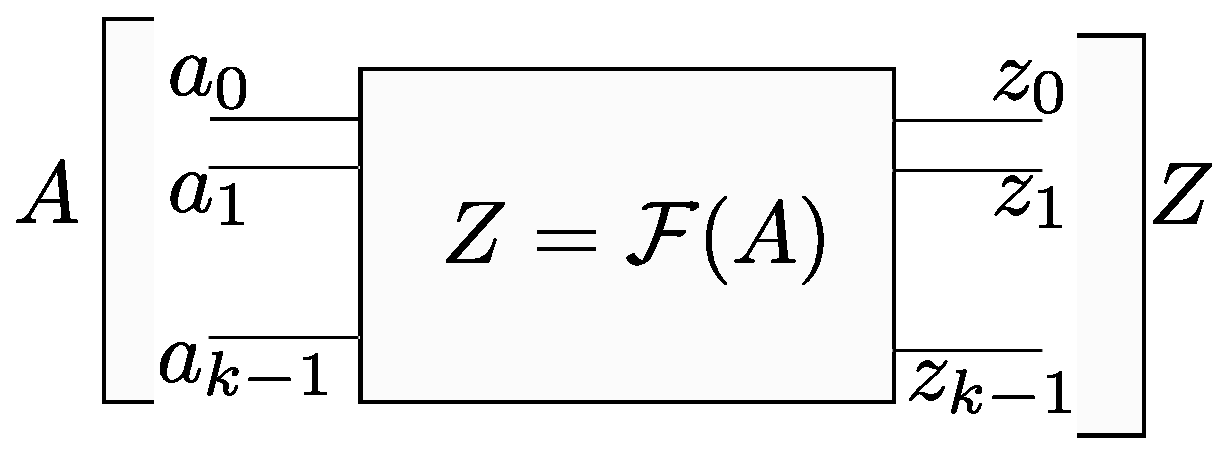
\includegraphics[width=0.5\textwidth]{./figures/interpolate}
}
\caption{Derive the abstraction $Z=\Func(A)$}
\label{fig:abstractA_Z2}
\end{figure}
}

By modelling the the arithmetic circuit as a polynomial system in
$\Fkk[x_1,x_2,\cdots,x_d]$, the abstraction problem 
can be solved using a \Grobner basis computation using an
abstraction term order. 
However, as computing a \Grobner basis is computationally
expensive, this approach is directly  applicable only to Galois field arithmetic
circuits no larger than $40$-bits.

\section{Problem Statement}

\begin{itemize}
\item  Given a gate-level combinational, acyclic circuit $C$ with $n$ word-level
$k$-bit inputs,
$A_1,\dots, A_n \in \Fkk$
and one $k$-bit output $Z$.
\item Pick a primitive, irreducible polynomial $P(x)$ over $\F_2[x]$ of degree $k$ 
to construct $\Fkk$ (these polynomials are known).
Let $P(\alpha) = 0$, where $\alpha \in \Fkk$ is a root of the irreducible
polynomial $P$.
\item The bit-level primary inputs of the circuit are denoted
$\{a_{0}^{i},a_{1}^{i},\dots,a_{k-1}^{i}\}$, for $1\leq i \leq n$;
the bit-level primary outputs are $\{z_0, \dots, z_{k-1}\} = Z$. 
Note that all $a_{j}^{i}, z_j \in \F_2$ for $0\leq j < k$.
\item Find the word-level polynomial function $\Func$ over $\Fkk$ 
computed by $C$ in the form of $Z=\Func(A_1, \dots, A_n)$.
\end{itemize}

In order for a combinational circuit $C$ to compute a function $f$ over the 
Galois field $\Fkk$, $C$ must have any number of 
$k$-bit word-level inputs and one $k$-bit word-level output.
Since every function over $\Fkk$ is a polynomial function, 
$C$ has a word-level polynomial representation over $\Fkk$.
The goal is to derive this word-level polynomial representation $\Func$ 
computed by a given combinational circuit over a 
given $\Fkk$.

%The proposed approach is generic enough to abstract the implementation of any
%combinational Galois field arithmetic circuit.
For the purpose of explaining the proposed abstraction approach, 
this chapter explores its application to Galois field multiplier circuits, 
which are described in Chapter \ref{ch:prelim}, 
as they form the core of most cryptographic computations in ECC and are 
notoriously hard to verify. In this case, $P(x)$ is chosen to be the same
primitive polynomial over which the circuit was designed.

\begin{Example}
Consider our problem statement as it applies to a multiplier 
circuit over $\Fkk$. The specification of the circuit is unknown.
\begin{itemize}

\item Given the Galois field $\Fkk$ and the corresponding
  irreducible polynomial $P(x)$. Let $P(\alpha) = 0$.

\item  Given a gate-level combinational circuit. The bit-level primary
  inputs of the circuit are $\{a_0, \dots, a_{k-1}, ~b_0, 
  \dots, b_{k-1}\}$, and the bit-level primary outputs are 
$\{z_0, \dots, z_{k-1}\}$; thus all $a_i, b_i, z_i \in \F_2$.

\item $A$ and $B$ denote the $k$-bit word-level inputs and $Z$ is the
$k$-bit word-level output. Therefore, 
$A = a_0 + a_1\alpha + \dots + a_{k-1}\alpha^{k-1}$,
$B = b_0 + b_1\alpha + \dots + b_{k-1}\alpha^{k-1}$, and 
$Z = z_0 + z_1\alpha + \dots + z_{k-1}\alpha^{k-1}$ with $A,B,Z \in \Fkk$.

\item Find the word-level polynomial function $\Func$ that this circuit 
implements over $\Fkk$.
The polynomial must be in the form of $Z=\Func(A,B)$. Since, in this case, 
the circuit is a multiplier, this resulting polynomial will be $Z=A\cdot B$.

\end{itemize}
\end{Example}

\section{Circuit Polynomial Modeling}

Given a gate-level implementation of a circuit,
we map each gate-level
Boolean operator in the circuit ($NOT$, $AND$, $OR$, $XOR$) to a polynomial 
over $\F_2$ using the following
one-to-one mapping over $\mathbb{B} \rightarrow \mathbb{F}_2$ : 
\begin{equation}
\label{b2poly}
\begin{split}
NOT :&~\neg a \rightarrow a+1 \pmod 2  \\   
AND :&~a \wedge b \rightarrow a\cdot b \pmod 2  \\ 
OR :&~a \vee b \rightarrow a+b+a\cdot b \pmod 2  \\
XOR :&~a \oplus b \rightarrow a+b \pmod 2 
\end{split}
\end{equation}
where $a,b \in \mathbb{F}_{2}=\{0,1\}$.
Note that the equation $c=\mathcal{F}(a,b)$ is written in polynomial
form as $c-\mathcal{F}(a,b)=c+\mathcal{F}(a,b)=0$, ~as $-1 \equiv +1
\pmod 2$.

\begin{Example}
Consider the equation with Boolean operators: 
\begin{equation}
z=a \oplus (b \vee c). \nonumber
\end{equation}

This equation modeled over $\F_2$ is:
\begin{equation}
z+a + b + c + b\cdot c=0 \nonumber
\end{equation}

Notice that the left-hand side expression is a polynomial in
$\F_{2}\left[a,b,c,z\right] \subset
\Fkk\left[a,b,c,z\right]$
\end{Example}

Secondly, we model the $k$-bit word-level inputs
and the $k$-bit word-level output of the given circuit as polynomial
expressions in $\mathbb{F}_{2^{k}}$ as shown in the problem statement.
If the $k$-bit word-level output of the circuit is denoted $Z$ which is 
composed of bit-level outputs 
$z_0, \dots , z_{k-1}$, the corresponding equation
is:
\begin{equation}
 Z = z_0 + z_1 \alpha + \dots + z_{k-1} \alpha^{k-1} \nonumber
\end{equation}
Once again, since $-Z = +Z \pmod 2$, this equation is modelled as:
\begin{equation}
Z + z_0 + z_1 \alpha + \dots + z_{k-1} \alpha^{k-1} = 0 \nonumber
\end{equation}

Likewise, for all word-level inputs $A_1,\dots,A_n$ we have
\begin{eqnarray}
A_1 + a_0^1 \alpha + \dots + a_{k-1}^1 = 0 \nonumber \\
\vdots \nonumber \\
A_n + a_0^n \alpha + \dots + a_{k-1}^n = 0 \nonumber 
\end{eqnarray}

Overall, a combinational circuit composed of $s$ Boolean gates
with $n$ $k$-bit inputs, $A_1, \dots , A_n$, and one $k$-bit output $Z$, 
is modeled as a polynomial system over $\mathbb{F}_{2^{k}}$ as follows:  

\begin{eqnarray}
 \left .  \begin{aligned}
f_1(x_1,x_2,\cdots, x_d)=0  \\
f_2(x_1,x_2,\cdots, x_d)=0  \\
\vdots  \\
f_s(x_1,x_2,\cdots, x_d)=0 \\
\end{aligned} 
\ \right\}
 &\qquad&  \text{\it Bit-level circuit constraints} \nonumber \\
 \left . \begin{aligned}
f_{Z}: Z+z_{0}+z_{1}\cdot \alpha,\cdots,{z_{k-1}}\cdot \alpha^{k-1}=0    \\
f_{A_1}:A_1+a_{0}^1+a_{1}^1\cdot \alpha+\cdots+a_{k-1}^1\cdot \alpha^{k-1}=0   \\
\vdots  \\
f_{A_n}:A_n+a_{0}^n+a_{1}^n\cdot \alpha+\cdots+a_{k-1}^n\cdot \alpha^{k-1}=0   \\
\end{aligned} 
\right\}
 &\qquad&  \text{\it Word-level designation} \nonumber \\
\end{eqnarray}


\begin{Example}
\label{exp:mul2bit}
Consider a 2-bit multiplier over ${\mathbb{F}}_{2^2}$ with
$P(x)=x^{2}+x+1$, given in Fig. \ref{fig:2bitmul}. Variables $a_0,
a_1, b_0, b_1$ are primary inputs, $z_0, z_1$ are primary outputs, and
$c_0, c_1, c_2, c_3, r_0$ are intermediate variables. 
%The gate $\otimes$
%corresponds to AND-gate, i.e. bit-level multiplication modulo 2. The
%gate $\oplus$ corresponds to XOR-gate, i.e. addition modulo 2.

\begin{figure}[H]
\centerline{
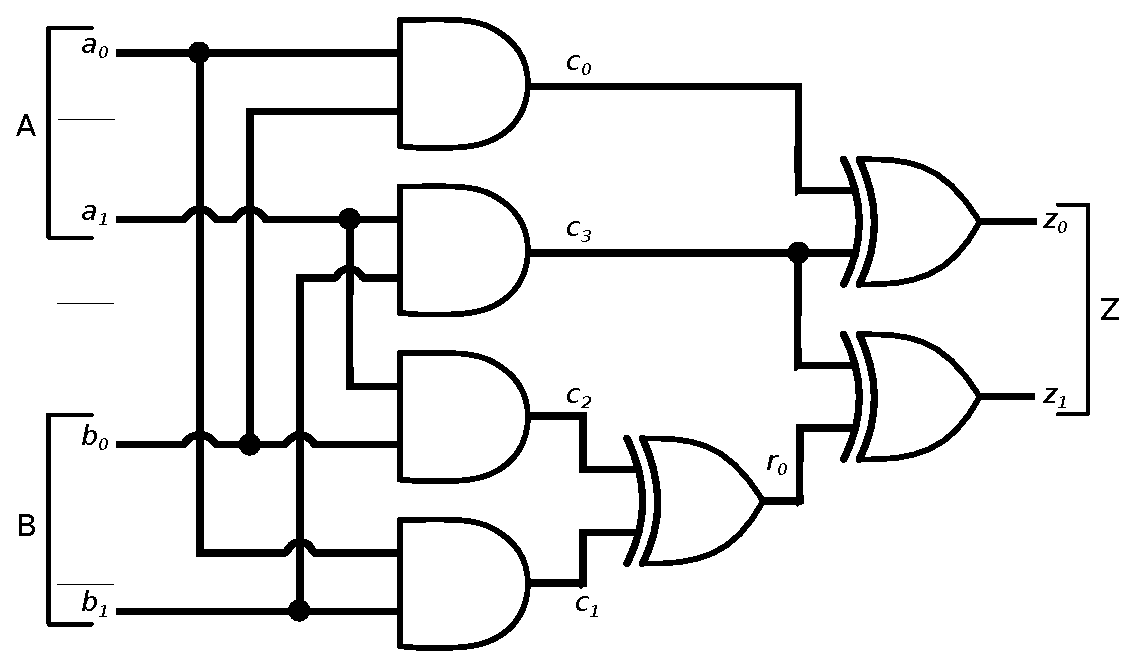
\includegraphics[scale=0.4]{./figures/2bitmasmult.eps}
}
\caption{ A 2-bit multiplier over ${\mathbb{F}}_(2^2)$.}
\label{fig:2bitmul}
\end{figure}

The circuit can be described using the following Boolean equations:
\begin{align*}
c_0=a_0 \wedge b_0,   \nonumber \\
c_1=a_0 \wedge b_1,   \nonumber \\
c_2=a_1 \wedge b_0, \nonumber \\
c_3=a_1 \wedge b_1,   \nonumber \\
r_0=c_1 \oplus c_2 ,      \nonumber \\
z_0=c_0 \oplus c_3,   \nonumber \\
z_1=r_0 \oplus c_3,    \nonumber
\end{align*}

With the mapping rules given in Equation \ref{b2poly}, 
the above equations are transformed into the following polynomials:
\begin{align*}
c_0+a_0 \cdot b_0,   \nonumber \\
c_1+a_0 \cdot b_1,   \nonumber \\
c_2+a_1 \cdot b_0,   \nonumber \\
c_3+a_1 \cdot b_1,   \nonumber \\
r_0+c_1 + c_2 ,      \nonumber \\
z_0+c_0 + c_3,   \nonumber \\
z_1+r_0 + c_3,   \nonumber
\end{align*}

Therefore, our overall polynomial system is:
\begin{eqnarray}
 \left .  \begin{aligned}
f_1: c_0+a_0 \cdot b_0  \\
f_2: c_1+a_0 \cdot b_1  \\
f_3: c_2+a_1 \cdot b_0  \\
f_4: c_3+a_1 \cdot b_1  \\
f_5: r_0+c_1 + c_2		\\
f_6: z_0+c_0 + c_3		\\
f_7: z_1+r_0 + c_3		   
 \end{aligned} 
\ \right\}
 &\qquad&  {\text {\it Bit-level circuit constraints}} \nonumber \\
 \left . \begin{aligned}
f_{A}: A+a_0+a_1\cdot \alpha  \\ 
f_{B}: B+b_0+b_1\cdot  \alpha  \\
f_{Z}: Z+z_0+z_1\cdot \alpha
 \end{aligned} 
\right\}
 &\qquad&  {\text {\it Word-Level designation}} \nonumber \\
\end{eqnarray}

\end{Example}

\section{Abstraction Formulation}

Let $S$ be the system of 
polynomials, 
$\{f_1,\dots,f_s,f_{A_1},\dots,f_{A_n},f_{Z}\}\subset \Fkk$, 
derived from the hardware
implementation of the Galois field arithmetic circuit over $\Fkk$.
This circuit performs some unknown function $f$ over 
$\Fkk$ in the form of $Z=\Func(A_1,\dots,A_n)$, where $Z$ is the $k$-bit 
output and $A_1,\dots,A_n$ are the $k$-bit inputs.
The polynomial representation of $\Func$ over $\Fkk$ is thus:

\begin{equation}
f_{\Func}: Z+\Func(A_1,\dots,A_n) \nonumber
\end{equation}

Since $f_{\Func}$ is ultimately derived from the circuit implementation, 
it agrees with the solution to the system of polynomials $\{S\}=0$, i.e.:
\begin{equation}
f_1=\dots=f_s=f_{A_1}=\dots=f_{A_n}=f_{Z}=0 \nonumber
\end{equation}
Thus, if we let $J=\langle f_1,\dots,f_s,f_{A_1},\dots,f_{A_n},f_{Z}\rangle$ 
be the ideal generated by $S$, 
$f_{\Func}$ {\bf vanishes} on the variety $V_{\Fkk}(J)$. 
Therefore, due to Proposition \ref{pro:iofv}, 
$f_{\Func}$ must be contained in the ideal of polynomials that vanish on
this variety, $f_{\Func} \in I(V_{\Fkk}(J))$. 

By applying Strong Nullstellensatz over $\Fkk$ (Theorem \ref{thm:sns}), 
$I(V_{\Fkk}(J))=J+J_0$ where
$J_0$ is the ideal generated by all vanishing polynomials in $\Fkk$. 
Recall that a vanishing polynomial in $\Fkk[x]$ is $x^q-x=x^q+x$. 
In our case, 
$\{x_1,\dots,x_d\} \in \F_2$ and $\{A_1,\dots,A_n,Z\} \in \Fkk$.
Thus, for $\Fkk[x_1,\dots,x_d,A_1,\dots,A_n,Z]$: 
\begin{equation}
J_0 = \langle x_1^2+x_1,\dots,x_d^2+x_d, A_1^{2^k}+A_1,\dots,A_n^{2^k}+A_n,Z^{2^k}+Z\rangle \nonumber
\end{equation}

The generators of the ideal sum $J+J_0$ are simply the combination of the 
generators of $J$ and the generators $J_0$.

\begin{Example}
\label{exp:finalMul2Bit}
Let us re-consider Example \ref{exp:mul2bit}. First, polynomials are
extracted from the circuit implementation as
shown in Example \ref{exp:mul2bit}. These polynomials represent the
ideal $J$. Along with the ideal of vanishing polynomials $J_0$, 
the following polynomials represent the generators 
of $J+J_0$ for the multiplier circuit. 

\begin{eqnarray}
 \left .  
	\begin{aligned}
		f_1:c_0+a_0 \cdot b_0  \\
		f_2:c_1+a_0 \cdot b_1  \\
		f_3:c_2+a_1 \cdot b_0  \\
		f_4:c_3+a_1 \cdot b_1  \\
		f_5:r_0+c_1 + c_2		\\
		f_6:z_0+c_0 + c_3		\\
		f_7:z_1+r_0 + c_3		
	\end{aligned} 
 \ \right\}
 &\qquad&  {\it  \text{Bit-level circuit constraints} ~(\subset J)} \nonumber \\
 \left . 
	\begin{aligned}
		f_{A}:A+a_0+a_1\cdot \alpha   \\ 
		f_{B}:B+b_0+b_1\cdot \alpha  \\ 
		f_{Z}:Z+z_0+z_1\cdot \alpha   
	\end{aligned} 
 \right\}
 &\qquad&  {\it  \text{Word-level designation} ~(\subset J)} \nonumber \\
  \left . 
	\begin{aligned}
		a_0^2-a_0, ~a_1^2-a_1,~b_0^2-b_0, ~b_1^2-b_1   \\ 
		c_0^2-c_0, ~c_1^2-c_1,~c_2^2-c_2, ~c_3^2-c_3  \\ 
		r_0^2-r_0, ~z_0^2-z_0,~z_1^2-z_1    \\ 
		A^4-A, ~B^4-B ,~Z^4-Z		  
	\end{aligned} 
 \right\}
 &\qquad&  {\it \text{vanishing polynomials} (J_0)} \nonumber
\end{eqnarray}
 
\end{Example}

The variety $V_{\Fq}(J)$ is
the set of all consistent assignments to the nets (signals) in the
circuit $C$. If we {\it project this variety on the word-level input and
output variables of the circuit $C$, we essentially generate the
function $\Func$ implemented by the circuit.} Projection of varieties from
$d$-dimensional space $\Fq^d$ onto a lower dimensional subspace
$\Fq^{d-l}$ is equivalent to {\it eliminating $l$ variables} from the
corresponding ideal. This can be done by computing a \Grobner basis
of the ideal with elimination ordering, as described in the 
Elimination Theorem (Theorem \ref{thm:elimth}).
Thus, we can find the polynomial 
$f_\Func:Z+\Func(A_1,\dots,A_n)$ by computing the \Grobner
basis of $J+J_0$ using the proper elimination ordering.

The proposed elimination order for 
abstraction is defined as the {\bf abstraction term order}. 

\begin{Definition}
\label{def:ato}
Given a circuit $C$,
let $x_1, \dots, x_d$ denote all the bit-level variables, 
let $A_1,\dots,A_n$ denote the $k$-bit word-level inputs, 
and let $Z$ denote the $k$-bit word-level output. 
Using the partial variable order 
$\{x_1, \dots, x_d\} > Z > \{A_1, \dots, A_n\}$,
where any refinement of the order will do,
impose a lex term order $>$ on the polynomial ring 
$R = \Fq[x_1, \dots, x_d, Z, A_1, \dots, A_n]$. 
This elimination term order $>$ is defined as
the {\bf Abstraction Term Order}. The relative ordering among $x_1,
\dots, x_d$ is not important and can be chosen arbitrarily. Likewise,
the relative ordering among $A_1, \dots, A_n$ is also unimportant.
\end{Definition}

\begin{Theorem}
{\bf Abstraction Theorem:} Using the setup and notations above,
compute a \Grobner basis $G$ of ideal $(J+J_0)$ using the abstraction term 
order $>$. Then: \\
(i) For every word-level input $A_i$, $G$ must contain the vanishing 
polynomial $A_i^q - A_i$ as the only polynomial with $A_i$ as its only 
variable;\\
(ii) $G$ must contain a polynomial of the form 
$Z + \mathcal{G}(A_1,\dots,A_n)$; and\\ 
(iii) $Z + \mathcal{G}(A_1,\dots,A_n)$ is such that 
$\Func(A_1,\dots,A_n) = {\mathcal{G}}(A_1,\dots,A_n),
\forall A_1,\dots,A_n \in \Fq$. 
In other words, ${\mathcal{G}}(A_1,\dots,A_n)$ and $\Func(A_1,\dots,A_n)$ are
equal as polynomial functions over $\Fq$.
\label{thm:abs}
\end{Theorem}

\begin{Proof}\
(i) For $A_i$, $A_i^q-A_i$ is a given generator of $J_0$. 
  $A_1,\dots,A_n$ are also 
  the last variables in the abstraction term order. Moreover, $A_i$ is an
  input to the circuit, so $A_i$ is an independent variable. As a result, 
  $G_{d+1} = G \cap\Fkk[A_1,\dots,A_n] = \{A_1^q - A_1,\dots,A_n^q-A_n\}$.

(ii) Since $f:Z + \Func(A_1,\dots,A_n)$ is a polynomial representation of
  the function of the circuit, $Z + \Func(A_1,\dots,A_n) \in J + J_0$, as
  described above. Therefore, according to the definition of a
  \Grobner basis, the leading term of $Z +
  \Func(A_1,\dots,A_n)$ (which is $Z$) should be divisible by the leading
  term of some polynomial $g_i \in G$. The only way $lt(g_i)$ can
  divide $Z$ is when $lt(g_i) = Z$ itself. Moreover, due to our
  abstraction (lex) term order, $Z > A > \dots > A_n$, so this polynomial 
  must be of the form $Z + {\mathcal{G}}(A_1,\dots,A_n)$. 

(iii) As $Z = \Func(A_1,\dots,A_n)$ represents the function of the circuit, 
  $Z + \Func(A_1,\dots,A_n) \in J + J_0$. 
  Moreover, $V(J + J_0) \subset V(Z + \Func(A_1,\dots,A_n))$. 
  By projecting this variety $V(J + J_0)$ onto the co-ordinates
  corresponding to $(A_1,\dots,A_n, Z)$, we obtain the {\it graph of the
  function} $(A_1,\dots,A_n) \mapsto \Func(A_1,\dots,A_n)$ 
  from $\Fkk \rightarrow \Fkk$. Since $Z + {\mathcal{G}}(A)$ is an element 
  of the \Grobner basis of $J + J_0$, 
  $V(J + J_0) \subset V(Z + {\mathcal{G}}(A_1,\dots,A_n))$. Therefore,
  $Z = {\mathcal{G}}(A_1,\dots,A_n)$ gives the same function as 
  $Z = \Func(A_1,\dots,A_n)$, for all $A_i \in \Fkk$.
\end{Proof}

As a consequence of the Abstraction Theorem, computing a \Grobner
basis $G$ of $J + J_0$ using the abstraction term order finds
a polynomial of the form $Z + \G(A_1,\dots,A_n)$ in the \Grobner basis, 
such that $Z = \G(A_1,\dots,A_n)$ is a polynomial representation of the 
circuit. However, if the \Grobner basis is not reduced, it is possible to 
obtain multiple polynomials in $G$ of the form 
$Z + \G _1(A_1,\dots,A_n), Z + \G _2(A_1,\dots,A_n), \dots,$;
all of which correspond to the same function. 

\begin{Corollary}
By computing a {\bf reduced} \Grobner basis $G_r$ of $J + J_0$, 
$G_r$ will contain one and only one polynomial in of the form 
$Z + \G(A_1,\dots,A_n)$, such that $Z = \G(A_1,\dots,A_n)$ is the 
{\bf unique, minimal, canonical} representation of the function 
$\Func$ implemented by the circuit.  
\end{Corollary}

\begin{Proof}
Any function $f: \Fkk^d \to \Fkk$ has a unique canonical 
representation as polynomial $P_f \in \Fkk[x_1, ..., x_d]$ such that all 
its nonzero monomials are of the form $x_1^{i_1}\cdots x_d^{i_d}$ where $0 
\leq i_j \leq q-1$, for all $j=1, \ldots d$.

%Let $q_i$ be a power of $2$ for $i=1, \ldots, d$. 
Let $J_0$ be the 
ideal of all polynomials that vanish over $\Fkk[x_1, \ldots, x_d]$.
The generators of $J_0$ are polynomials in the form $x_i^{2^q_i}-x_i$,
where $q_i$ is the datapath size of $x_i$.
Then these generators also form a reduced Gr\"obner basis for $J_0$.
This implies that the elements $A_h^{2^k}-A_h, 1 \leq h \leq n$ will 
have to be part of the reduced Gr\"obner basis of $J+J_0$.

Corollary 1.8.6 in~\cite{gb_book} shows that the obtained element $\Func
(A_1,..., A_n)$ that is reduced modulo
$A_h^{2^k}-A_h, 1 \leq h \leq n$. Thus, the polynomial representation of 
$\Func$ in the reduced \Grobner basis is the unique canonical 
representation.
\end{Proof}

\begin{Example}
Consider the $2$-bit multiplier Example 
\ref{exp:finalMul2Bit}, for which we have already generated $J+J_0$. 
We apply abstraction term order $>$, i.e a lex order with
"bit-level variables" $>$ "Output Z" $>$ "Inputs A, B".

When we compute the reduced \Grobner basis, $G_r$, of \{$J + J_0$\} with 
respect to this ordering, $G_r$ = \{$g_1, \dots, g_{14}\}:$
\begin{align*}
g_1: B^4+B; 
~~g_2: b_0+b_1 \alpha + B; 
~~g_3: a_0+a_1 \alpha + A;  \nonumber \\
~~g_4: c_0+c_1 \alpha + c_2 \alpha + c_3(\alpha+1)+Z;
g_5: r_0+c_1+c_2; 
~~g_6: z_0+c_0+c_3; \nonumber \\
~~g_7: z_1+r_0+c_3; 
~~{\bf g_8: Z+A\cdot B};
~~g_9: b_1+B^2+B; 
~~g_{10}: a_1+A^2+A; \nonumber \\
~~g_{11}: c_3+a_1\cdot b_1
g_{12}: c_2+a_1\cdot b_1 \alpha + a_1 \cdot B; 
~~g_{13}: c_1+a_1\cdot b_1 \alpha +b_1 A; 
~~g_{14}: A^4+A  \nonumber
\end{align*}

$g_8=Z+A\cdot B$ is the {\bf canonical, word-level polynomial } 
representing the function performed by the multiplier $Z=A\cdot B$.
\end{Example}

Consolidating our results, the proposed abstraction approach is described
as follows: 

\begin{enumerate}
\item Given a bit-level implementation of a Galois field arithmetic circuit 
$C$ over a given $\Fkk$, 
with $k$-bit output $Z$ and $k$-bit inputs $A_1,\dots,A_n$. 
\item $C$ performs some unknown function $Z=\Func(A_1,\dots,A_n)$.
\item Model the the circuit as a system of polynomials 
$\{f_1,\dots,f_s\}\subset \Fkk[x_1,\dots,x_d, Z, A_1, \dots, A_n]$ as 
described above and let $J$ be the ideal generated by these polynomials. 
\item Let $J_0$ be the ideal generated by all vanishing polynomials of 
$\Fkk$. 
\item By computing a reduced \Grobner basis $G_r$ of ideal $J+J_0$ using 
{\bf abstraction term order}, 
the word-level polynomial $Z+\Func(A_1,\dots,A_n)$ will be found in $G_r$.
\end{enumerate}

\section{Experimental Results: Validation of the Approach}

Our experiments take, as inputs, Mastrovito \cite{mastro:1989} multiplier 
circuits of various word sizes $k$. Each multiplier performs the polynomial 
function $Z = \Func(A,B) = A \cdot B$ over a Galois field, 
where $Z$ is the $k$-bit 
output and $A$ and $B$ are the $k$-bit inputs. We extract the 
Boolean gate-level operators $J$ and vanishing polynomials $J_0$.
Then we compute the reduced \Grobner basis $G_r$ of $J + J_0$
with respect to abstraction term order $>$. The resulting $G_r$ contains a 
polynomial $Z + A\cdot B$. 

The experiments were designed as scripts in the computer algebra tool, 
{\sc Singular} \cite{DGPS}, which provides functionality for polynomial
computations over rings and fields. This tool provides a number of efficient 
polynomial algorithms. The ring $\Fkk[x_1,\dots,x_f,\allowbreak Z,A,B]$ is defined over
the abstraction ordering, using the same primitive polynomial 
(``minpoly'' in Singular) $P(X)$ that was used to design the Galois field multiplier. 
Ideals  $J$ and $J_0$ were provided using their generating polynomials and the
the reduced \Grobner basis computation of $J+J_0$ was performed
using the ``slimgb'' command.

The experiments were conducted on a 64-bit Ubuntu machine running a 2.4GHz 
processor with 8GB of memory. We applied our approach to
abstract the canonical, polynomial representation of Mastrovito 
multipliers of various sizes.
Our machine was unable to perform the 
computations of the Gr\"obner basis of multipliers beyond $40$-bit word 
inputs. 

\begin{table}[H]
\label{tab:slimgb}
	\begin{center}
	    \caption{Run-time of Gr\"obner Basis Computation of Mastrovito Multipliers in Singular using Abstraction Term Order $>$.}\label{tab:sT}
	    \begin{tabular}{|c|c||c|} 
	        \hline
		Word Size ($k$) & Number of Polynomials ($d$) & Computation Time (minutes)   \\
		\hline
	        $16$	&  $1,871$  & $2.4$ \\
		$24$	&  $3,135$  & $12$  \\
	        $32$	&  $5,549$  & $22.6$ \\
	        $40$	&  $8,587$  & $266$ \\
		$48$	& $12,327$  & NA (Out of Memory) \\
	        \hline
	    \end{tabular}
	\end{center} 
\end{table}

\section{Conclusions}
The above approach is guaranteed to find a canonical, word-level 
representation of the function $\Func$ performed by a circuit $C$ over 
$\Fkk$. However, the \Grobner basis computation is prohibitively complex for
circuits of practical sizes. The next chapter proposes a 
method to overcome the complexity of the \Grobner
basis computation in order to make this abstraction approach scalable.
